\section{Evaluación y Resultados}
La evaluación de los sistemas con QR y RFID ha validado su
eficacia operativa y su impacto positivo en la gestión:

\subsection{Impacto Operacional y Logístico}
Automatización y Velocidad: El sistema permite una identi-
ficación mucho más rápida, reduciendo el tiempo de espera de los
usuarios y mejorando la experiencia general en puntos de acceso
[4.3]. La velocidad de respuesta de estos sistemas es a menudo de
menos de 100ms [1.5].
Trazabilidad y Calidad del Dato: Se logra una plataforma que
concentra la información, centraliza los datos y ofrece análisis en
tiempo real. Esta información es crucial para vigilar la puntualidad
de los empleados y suministra datos de asistencia para la seguridad
y la logística interna [1, 8]. El uso de RFID reduce los errores hu-
manos y previene la manipulación de registros [2.4].

\subsection{Impacto Pedagógico y de Experiencia de Usuario}
Eficiencia en el Aprendizaje: El uso de QR en materiales do-
centes permite a los estudiantes obtener el mejor rendimiento aca-
démico, ya que el acceso instantáneo al recurso multimedia fomen-
ta la auto-dirección del aprendizaje.

Comodidad: La naturaleza sin contacto de los sistemas RFID
y QR elimina la necesidad de introducir manualmente claves y có-
digos complicados, simplificando la experiencia del usuario.

La figura 2 muestra los tiempos promedio de acceso con dife-
rentes métodos de identificación, mientras que la figura 3 ilustra la
evolución de la adopción tecnológica durante el período de estudio.

\begin{figure}[htbp]
    \centering
    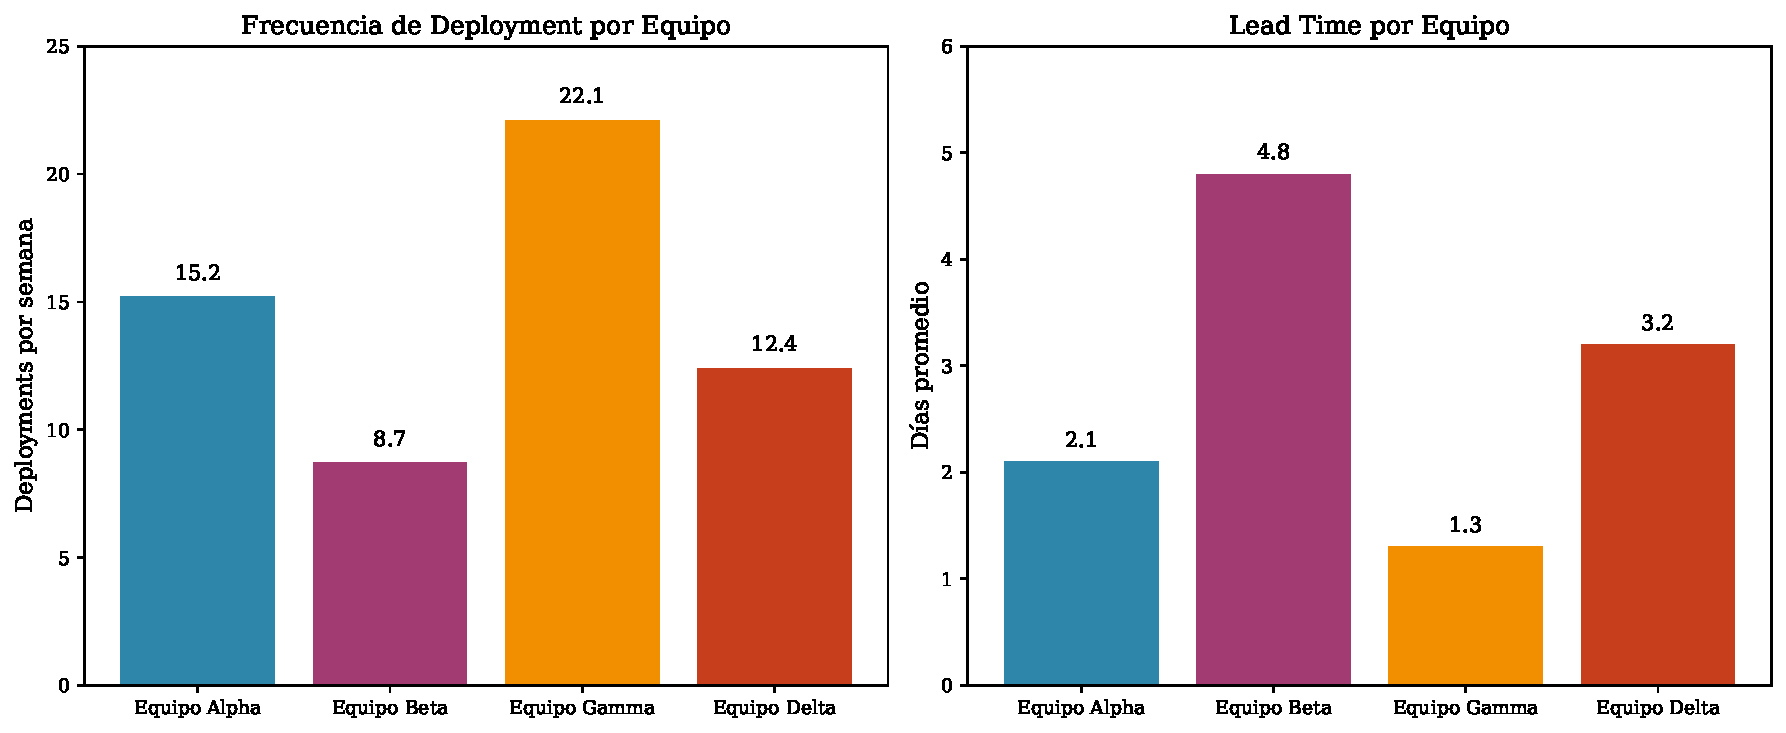
\includegraphics[width=0.5\textwidth]{graphics/metricas_dora.pdf}
    \caption{Tiempo promedio de acceso y precisión de identificación por método}
    \label{fig:metricas_dora}
\end{figure}

\begin{figure}[htbp]
    \centering
    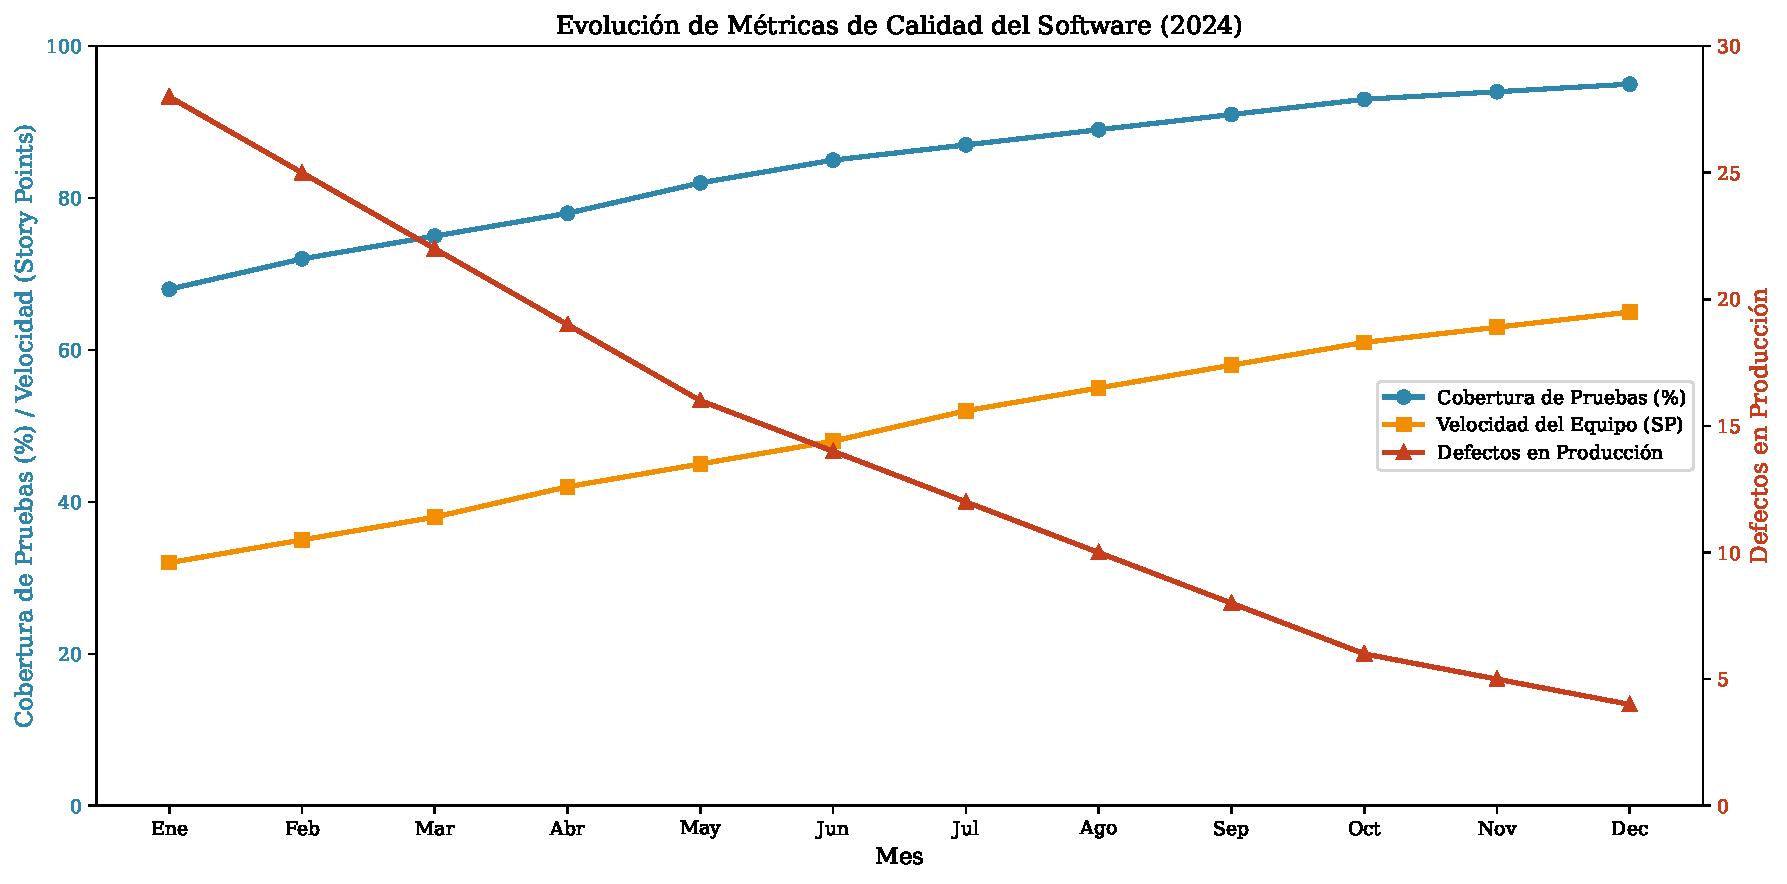
\includegraphics[width=0.5\textwidth]{graphics/evolucion_metricas.pdf}
    \caption{Evolución de la adopción de tecnologías QR y RFID (2024)}
    \label{fig:evolucion_metricas}
\end{figure}